
\section{Introdução}

  O analisador sintático é o responsável por reconhecer a estrutura da linguagem, formada a partir da gramática. Sua ação começa uma vez que o módulo léxico já reconheceu todas as partículas átomicas que compõem o código-fonte.


  Na realidade, é o analisador sintático quem invoca a ação do módulo léxico em um primeiro momento a fim de identificar as partículas do texto. A medida que os tokens são lidos e repassados ao analisador sintático, ele, o analisador sintático, tenta descrever como essas partículas estão estruturadas e organizadas no texto. A estrutura é chamada de árvore de sintaxe e consiste unicamente em uma forma alternativa de representar o código-fonte, mas a qual é compreensível pelo compilador.


  Em seguida, quando da análise semântica, é novamente o módulo sintático quem será o responsável por invocar o analisador semântico, o qual traduzirá a árvore de sintaxe em ações concretas, executáveis pelo computador.

        
  Outras funções tipicamente atribuídas ao analisador sintático são detecção de erros de sintaxe, recuperação de erros, correção de erros, ativação de rotinas de síntese do código-objeto, entre outras.


  Existem outras formas de delegar essas tarefas aos três módulos canônicos de um compilador clássico, mas podemos concluir que, por conta de nossas decisões de projeto, o compilador em desenvolvido é orientado à sintaxe. Isso porque o módulo sintático do compilador é o pivô central que coordena o fluxo sequencial de ações que permitem traduzir uma linguagem de alto nível em linguagem de máquina. É ele quem determina qual é a etapa do processo de compilação que está sendo executada e quem é o responsável por ela.

        
  Assim, após definir a linguagem e desenvolver o analisador léxico, tratamos de construir o módulo de análise sintática, cujo método de reconhecimento foi baseado em autômato de pilha estruturado (APE). 

\section{Geração Automática dos Autômatos}
  \subsection{Notação de Wirth Reduzida}

    Na primeira etapa para a criação do APE, foram utilizadas as expressões fundamentais criadas a partir da descrição reduzida em notação de Wirth. A definição das expressões seguiu o critério dos não-terminais com recursividade central, sendo possível concluir que as máquinas finais tratariam a sequência de comandos, as expressões e o programa principal.


    Assim, a linguagem representada pela notação de Wirth reduzida pode ser encontrada no arquivo "wirth\_reduzido.txt" que acompanha esse documento.
    

    %\lstinputlisting{../1-linguagem/notacoes/wirth_reduzido.txt}

  \subsection{Lista de submáquinas do APE}
    \subsubsection{Lista de transições}

      A partir da linguagem representada em notação de Wirth reduzida, utilizamos o programa do site indicado \footnote{http://radiant-fire-72.heroku.com/} para gerar automaticamente a tabela de transições as quais as submáquinas deveriam executar de forma a caracterizar a linguagem.


      O programa gera diversas tipos de saídas. Cuida lembrar que somente consideramos a saída que é uma tabela de transição reduzida, de forma a otimizar o processamento do compilador e facilitar a leitura e boa compreensão da representação dos autômatos, seja ela na forma tabular ou gráfica.


      Grosso modo, o programa utiliza três etapas para reduzir a tabela de transições. A ordem em que elas devem ser executadas é a seguinte:


      \begin{itemize}
        \item Eliminação das transiçõees em vazio;
        \item Eliminação dos estados não-acessíveis;
        \item Eliminação dos estados equivalentes.
      \end{itemize}


      A saída do tabela referente à submáquina programa:

      \lstinputlisting{../1-linguagem/notacoes/JFLAP/programa/programa.txt}


      A saída referente à submáquina comando:

      \lstinputlisting{../1-linguagem/notacoes/JFLAP/comando/comando.txt}

      
      E, finalmente, a saída referente à submáquina expressão:

      \lstinputlisting{../1-linguagem/notacoes/JFLAP/expressao/expressao.txt}

    \subsubsection{Lista dos autômatos}

      Nesta seção listaremos simplesmente os autômatos resultantes representados de uma maneira gráfica a partir das tabelas de transições da seção anterior.


      A ferramenta utilizada para gerar a modelagem gráfica é o JFLAP, obtido do site (http://www.cs.duke.edu/csed/jflap/)


      \begin{figure}[H]
        \caption{Autômato representando a submáquina programa}
        \centering
          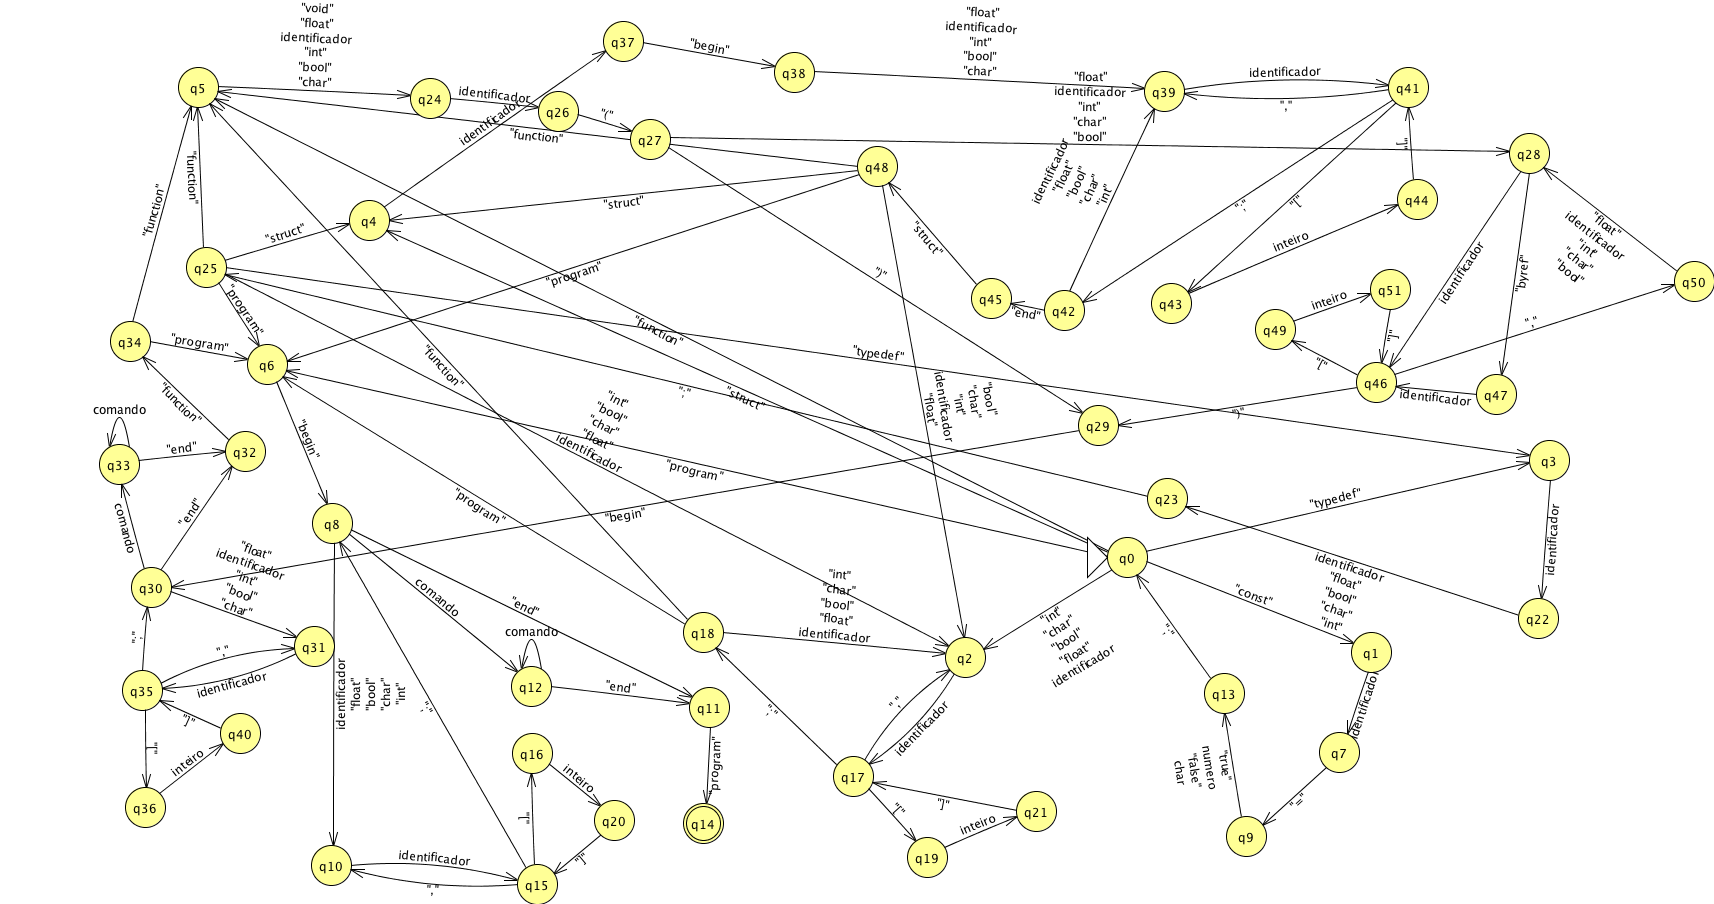
\includegraphics[width=0.7\textwidth]{../1-linguagem/notacoes/JFLAP/programa/programa.png}
      \end{figure}

      \begin{figure}[H]
        \caption{Autômato representando a submáquina comando}
        \centering
          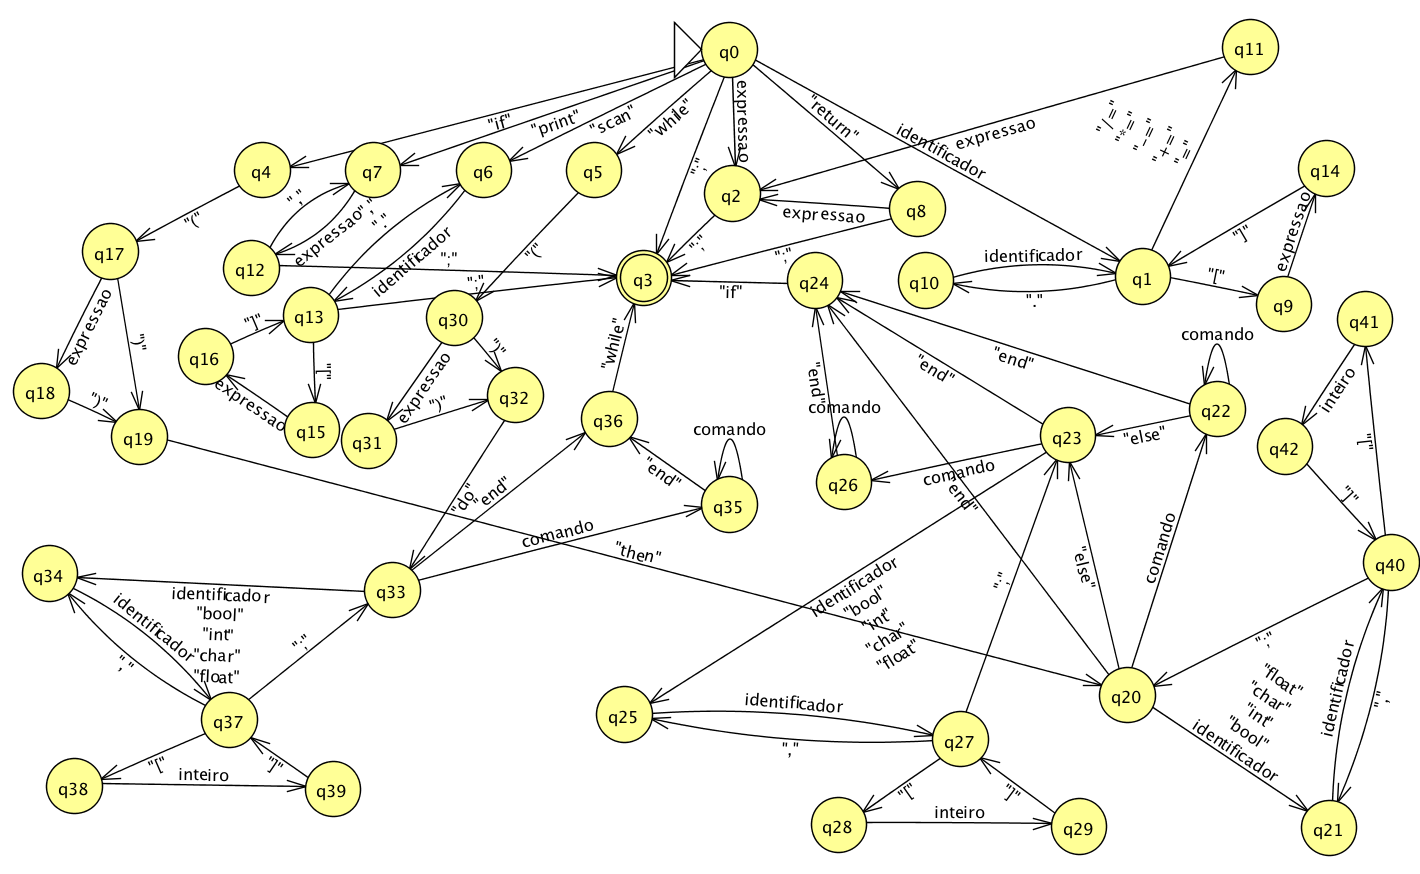
\includegraphics[width=0.7\textwidth]{../1-linguagem/notacoes/JFLAP/comando/comando.png}
      \end{figure}


      \begin{figure}[H]
        \caption{Autômato representando a submáquina expressao}
        \centering
          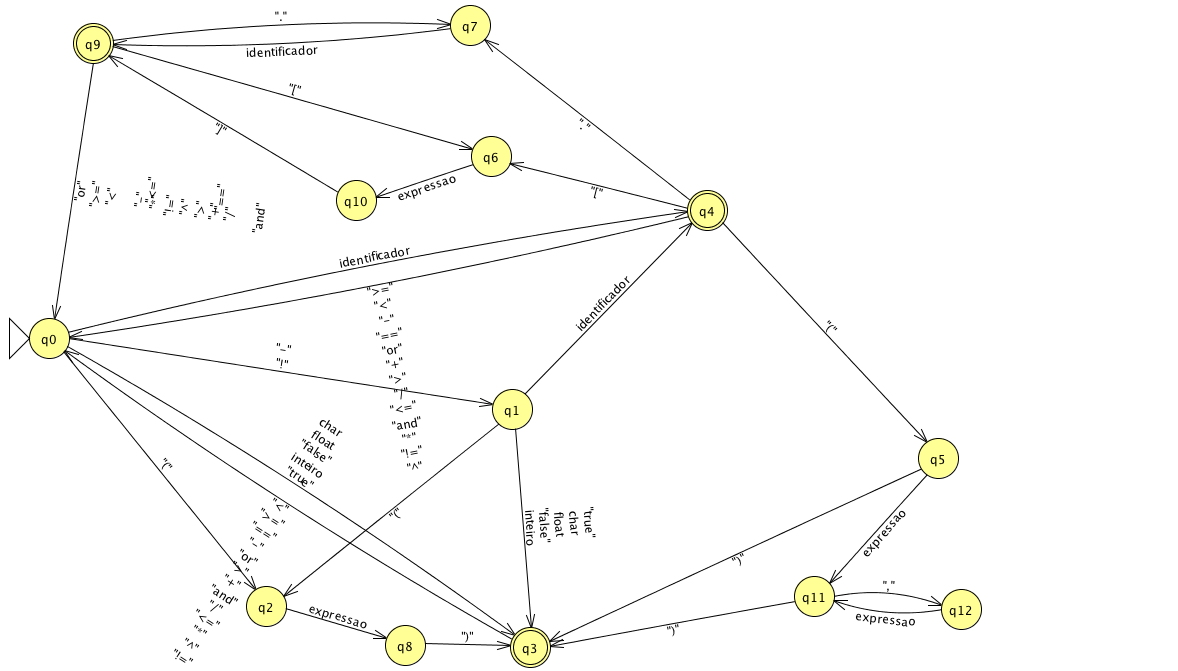
\includegraphics[width=0.7\textwidth]{../1-linguagem/notacoes/JFLAP/expressao/expressao.png}
      \end{figure}

\section{Comentários sobre a implementação}

  \subsection{Desenvolvimento do módulo sintático}


  Partindo do modelo da notação de Wirth reduzida, nosso analisador sintático baseia-se na interação entre três máquinas de estados, representando as regras finais, que podem se chamar mutuamente, o que é previsto por estarmos trabalhando com um Autômato de Pilha Estruturado (APE).


  O módulo sintático, portanto, começa suas atividades com a premissa que as três máquinas de estados já estejam criadas e inicializadas. Pressupõe-se que essa inicialização seja executada no programa principal (função main) do compilador.Essa inicialização ocorre de forma análoga ao que realizamos no módulo léxico e é baseada em tabelas de transições, as quais encontram-se descritas em arquivos externos, facilitando futuras modificações.

  
  Utiliza-se a subrotina verify\_syntax(), a qual já capaz de dizer se o compilador reconhece a linguagem. Mais detalhadamente, essa verificação tem como principal atividade o lançamento da função recognize(), utilizando a máquina que representa "programa`' e o primeiro token lido pelo analisador léxico como parâmetros.


  Grosso modo, o que esta função realiza é, dado o token passado via parâmetro, consulta-se sua tabela de transições internas e verifica-se se há alguma transição possível. Se sim, a transição é realizada, o estado do autômato é atualizado e um novo token é lido. 


  Cuida lembrar que há casos em que a transição chama uma nova submáquina, o que também é especificado pela tabela. Quando isso ocorre, a nova máquina é chamada através da mesma função regconize, mas passando a nova máquina como parâmetro e o mesmo token por referência. Em outros termos, não há necessidade de lookahead e, por serem armazenados em memória quando da chamada de submáquina, os tokens são consumidos sob demanda.


  Por outro lado, se não houver transição possível na tabela para um dado token, a função verifica se a máquina encontra-se em estado de aceitação, retornando verdadeiro, ou não, retornando falso. O valor falso traduz o caso em que houve um erro sintático na estrutura do código-fonte e o erro é rapidamento propagado para as máquinas de estados que a chamaram, parando a execução do módulo. Já o valor verdadeiro, faz com que a máquina que a chamou continue sua execução a partir do próximo estado previsto pela tabela em que o autômato estava a esperar (resincronização); se o autômato é a raiz ("programa`') e já não há mais tokens a serem lidos, o compilador reconhece a sintaxe da linguagem.


  \subsection{Integração com o compilador}


  Devido à alta modularização configurada pela arquitetura escolhida, o programa principal que representa o compilador possui uma estrutura bastante simples. 


  Primeiramente, o módulo léxico é inicializado, passando o código-fonte a ser analidado como parâmetro. Em seguida, inicializa-se a Tabela de Símbolos e a Tabela de Palavras-chaves. Até aqui, não há diferenças em relação à entrega do analisador léxico.


  A próxima ação, então, inicializa o módulo sintático, o que consiste basicamente na criação das máquinas de estados que representam as expressões de Wirth a partir dos arquivos externos, como descrito na seção anterior.

 
 Finalmente, chama-se a subrotina verify\_syntax(), a qual foi explicada anteriormente e é capaz de decidir se o código-fonte pertence ou não à lingugagem definida pela gramática.
